\documentclass[12pt,a4paper]{article}
\usepackage[utf8]{inputenc}
\usepackage[T1]{fontenc}
\usepackage{amsmath}
\usepackage{geometry}
\usepackage{setspace}
\usepackage{parskip}
\usepackage{enumitem}
\usepackage{booktabs}
\usepackage{longtable}
\usepackage{array}
\usepackage{xcolor}
\usepackage{hyperref}
\usepackage{float}
\usepackage{tikz}
\usetikzlibrary{arrows.meta,positioning,calc,matrix}
\usepackage{fancyhdr}
\usepackage{titlesec}

\geometry{left=2.5cm,right=2.5cm,top=2.5cm,bottom=2.5cm,headheight=14.5pt}
\onehalfspacing
\hypersetup{colorlinks=true,linkcolor=black,urlcolor=blue,pdftitle={Sistema Integral de Gestión de Eventos},pdfauthor={Samuel Contreras}}

\definecolor{azul}{RGB}{31,78,121}
\definecolor{gris}{RGB}{242,242,242}
\definecolor{grisoscuro}{RGB}{80,80,80}
\definecolor{verde}{RGB}{39,120,70}
\definecolor{naranja}{RGB}{230,126,34}
\definecolor{morado}{RGB}{106,27,154}

\titleformat{\section}{\Large\bfseries\color{azul}}{\thesection.}{0.5em}{}
\titleformat{\subsection}{\large\bfseries}{\thesubsection.}{0.5em}{}
% Etiquetas en español (sin babel, que no está disponible en este entorno)
\renewcommand{\contentsname}{Índice}
\renewcommand{\figurename}{Figura}
\renewcommand{\tablename}{Tabla}

\pagestyle{fancy}
\fancyhf{}
\fancyhead[L]{Sistema Integral de Gestión de Eventos}
\fancyhead[R]{Arquitectura de Software}
\fancyfoot[C]{\thepage}

\begin{document}

\begin{titlepage}
\centering
\vspace*{2cm}
{\Huge\bfseries Sistema Integral de Gestión de Eventos\par}
\vspace{0.7cm}
{\Large Arquitectura de Software\par}
\vspace{1.2cm}
{\Large\bfseries Atributos de Calidad y Propuesta Arquitectónica\par}
\vspace{2cm}
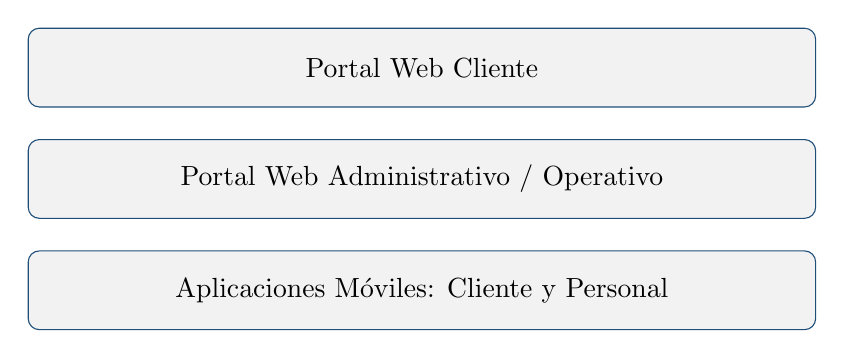
\begin{tikzpicture}
\node[draw=azul,rounded corners,fill=gris,minimum width=10cm,minimum height=1cm,align=center]
{Portal Web Cliente};
\node[draw=azul,rounded corners,fill=gris,minimum width=10cm,minimum height=1cm,below=0.4cm of current bounding box.south,align=center]
{Portal Web Administrativo / Operativo};
\node[draw=azul,rounded corners,fill=gris,minimum width=10cm,minimum height=1cm,below=0.4cm of current bounding box.south,align=center]
{Aplicaciones Móviles: Cliente y Personal};
\end{tikzpicture}
\vfill
\begin{tabular}{rl}
\textbf{Materia:} & Arquitectura de Software\\
\textbf{Estudiante:} & Samuel Contreras\\
\textbf{Fecha:} & Agosto de 2026
\end{tabular}
\end{titlepage}

\tableofcontents
\newpage

\section{Introducción}

Este documento presenta una segunda versión del análisis de atributos de calidad y de la propuesta de arquitectura para el \textbf{Sistema Integral de Gestión de Eventos}. La propuesta toma como base la primera versión del proyecto, donde se planteó una organización mediana-grande que gestiona eventos masivos, como conciertos, festivales y partidos deportivos, con miles de usuarios concurrentes, especialmente durante la apertura de venta y el ingreso al recinto.

El sistema centraliza procesos de boletería, mercado secundario de entradas, administración de personal, parqueaderos y operación de eventos. En esta segunda versión se define con mayor precisión la distribución de funcionalidades entre las interfaces.

Se contemplan cuatro clientes principales:

\begin{itemize}
\item \textbf{Portal Web del Cliente:} compra, consulta y gestión de entradas, reventas, promociones y parqueaderos.
\item \textbf{Portal Web Administrativo y Operativo:} utilizado por administradores, organizadores y trabajadores autorizados.
\item \textbf{Aplicación Móvil del Cliente:} principalmente para visualizar entradas y códigos QR, información y notificaciones.
\item \textbf{Aplicación Móvil del Personal:} para turnos, asistencia, instrucciones, reportes y alertas.
\end{itemize}

La primera propuesta priorizó consistencia, disponibilidad, seguridad y rendimiento. Esta versión mantiene esos atributos y aumenta la relevancia de tiempo real, trazabilidad, escalabilidad, usabilidad y portabilidad.

\section{Contexto y alcance}

El sistema está orientado a clientes, organizadores, administradores, supervisores, personal operativo y proveedores. Los principales dominios son:

\begin{enumerate}
\item Venta y gestión de boletería.
\item Mercado secundario de entradas.
\item Gestión de parqueaderos.
\item Logística y operación del evento.
\item Administración general.
\item Gestión del personal.
\item Gestión de emergencias y evacuaciones.
\end{enumerate}

La arquitectura debe permitir que estos dominios evolucionen de forma relativamente independiente y que los componentes con alta demanda puedan escalar sin afectar innecesariamente a los demás.

\section{Interfaces del sistema}

\subsection{Portal Web del Cliente}

El portal web permite registro e inicio de sesión, consulta de eventos, compra de entradas, consulta de entradas adquiridas, publicación y compra de entradas revendidas, cancelaciones y devoluciones, promociones, reserva de parqueadero y recepción de notificaciones.

La lógica de negocio crítica permanece en el backend y el portal consume los servicios mediante el API Gateway.

\subsection{Portal Web Administrativo y Operativo}

Está dirigido a administradores, organizadores y trabajadores autorizados. Incluye:

\begin{itemize}
\item CRUD de eventos, usuarios, clientes, empleados y roles.
\item CRUD de localidades y tipos de entrada.
\item CRUD de parqueaderos y zonas.
\item CRUD de proveedores, recursos logísticos y promociones.
\item Planificación de eventos.
\item Control de aforo.
\item Gestión de incidentes.
\item Gestión de emergencias y evacuaciones.
\item Monitoreo del evento.
\end{itemize}

\subsection{Aplicación Móvil del Cliente}

Permite iniciar sesión, consultar eventos y entradas, visualizar el código QR de cada entrada, consultar información del evento y recibir notificaciones y alertas. Su función crítica es facilitar el acceso rápido a los QR durante el ingreso.

\subsection{Aplicación Móvil del Personal}

Permite consultar eventos asignados, turnos, horarios y áreas de trabajo; confirmar asignaciones; solicitar cambios de turno; registrar ingreso y salida; recibir instrucciones; reportar incidentes y recibir alertas de emergencia.

\section{Atributos de calidad priorizados}

\begin{longtable}{p{2cm}p{3cm}p{9cm}}
\toprule
\textbf{Prioridad} & \textbf{Atributo} & \textbf{Justificación}\\
\midrule
Alta & Consistencia & Una entrada no puede pertenecer a dos propietarios ni venderse dos veces simultáneamente. También se requiere consistencia en pagos, transferencias, asignaciones y asistencia.\\
Alta & Disponibilidad & El sistema debe estar disponible durante ventas, ingreso masivo, operación del evento y emergencias.\\
Alta & Seguridad & Deben protegerse datos personales, credenciales, pagos, QR, información de empleados y permisos.\\
Alta & Rendimiento & Miles de usuarios pueden realizar operaciones concurrentes y las validaciones deben responder rápidamente.\\
Media-Alta & Tiempo real & Aforo, entradas, estado del personal, parqueaderos y emergencias deben actualizarse casi inmediatamente.\\
Media & Escalabilidad & Debe ser posible aumentar las instancias de los servicios con mayor demanda.\\
Media & Trazabilidad & Deben auditarse transferencias, pagos, accesos, turnos, operaciones administrativas y emergencias.\\
Baja-Media & Usabilidad & Las interfaces deben adaptarse a clientes, empleados, supervisores, organizadores y administradores.\\
Baja-Media & Mantenibilidad & Los cambios en un dominio no deberían afectar innecesariamente a los demás.\\
Baja-Media & Portabilidad & Las funcionalidades deben poder utilizarse mediante web y aplicaciones móviles.\\
Media & Integrabilidad & El sistema depende de dos integraciones externas críticas para el negocio (pasarela de pagos, proveedor de notificaciones) que deben poder cambiarse o fallar sin comprometer el flujo principal.\\
Media & Desplegabilidad & Los microservicios deben poder actualizarse (hotfixes, nuevas versiones) sin interrumpir un evento en curso, especialmente durante ingreso masivo o apertura de venta.\\
Media & Comprobabilidad & Los flujos críticos (reventa concurrente, pagos, protocolo de emergencia) deben poder probarse de forma aislada, sin depender de servicios externos reales.\\
Baja & Seguridad física (\textit{Safety}) & El sistema no controla hardware crítico, pero sí participa en la seguridad física de los asistentes a través del control de aforo y la coordinación de evacuaciones.\\
\bottomrule
\end{longtable}

Las cuatro filas añadidas (Integrabilidad, Desplegabilidad, Comprobabilidad y Seguridad física) corresponden a atributos vistos en el curso (Clases 7, 10, 11 y 13) que no estaban priorizados en la versión inicial de esta tabla; se incorporan aquí para que las tácticas y patrones aplicados en la Sección \ref{sec:tacticas-qa} tengan una prioridad explícita de la que derivarse, tal como exige el curso para todo el rango de clases 6 a 14.

\section{Arquitectura propuesta}

Se propone una arquitectura distribuida basada en \textbf{microservicios}, con API Gateway, balanceador de carga, Redis, RabbitMQ o Kafka y bases de datos independientes por dominio.

\begin{figure}[H]
\centering
\resizebox{\textwidth}{!}{
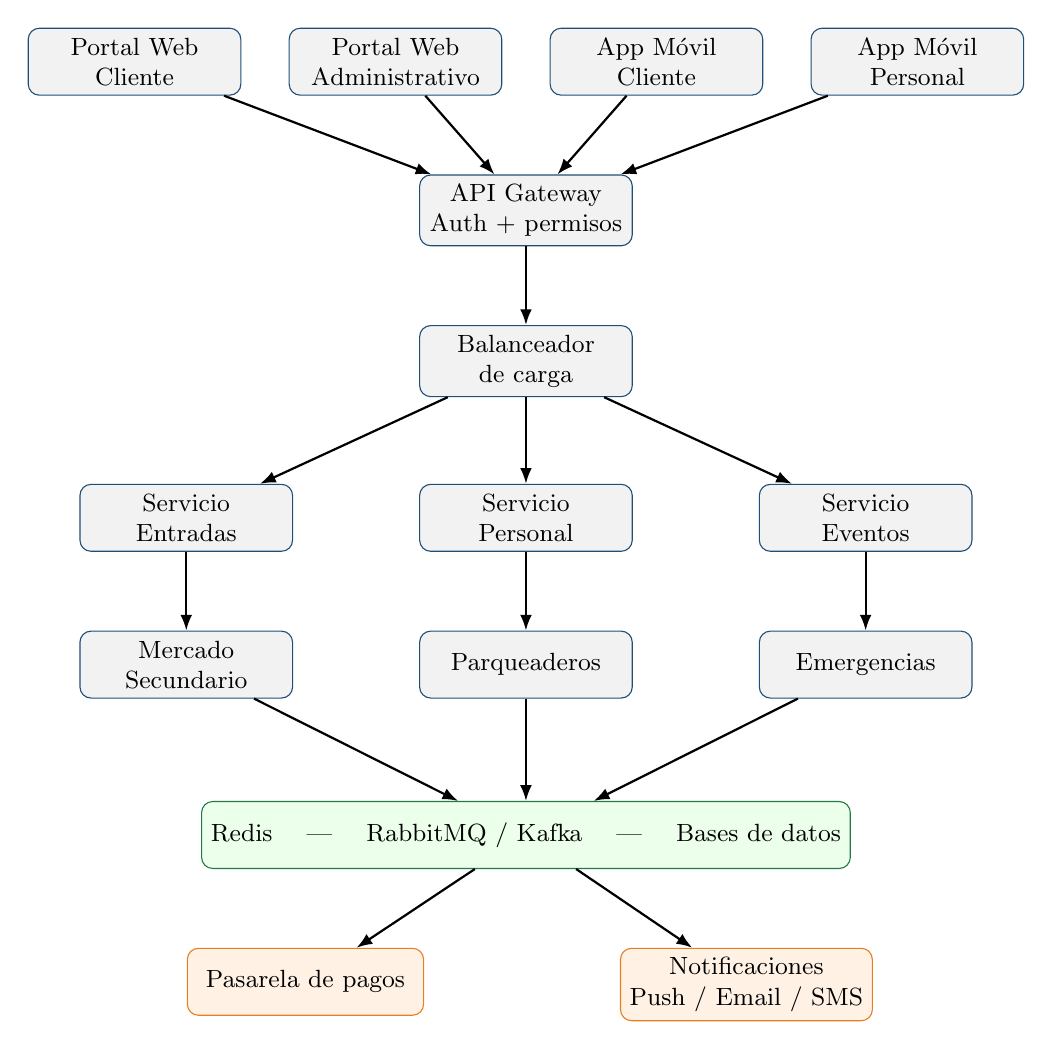
\begin{tikzpicture}[
box/.style={draw=azul,rounded corners,fill=gris,minimum width=2.7cm,minimum height=0.85cm,align=center,font=\small},
infra/.style={draw=verde,rounded corners,fill=green!8,minimum width=3cm,minimum height=0.85cm,align=center,font=\small},
ext/.style={draw=naranja,rounded corners,fill=orange!10,minimum width=3cm,minimum height=0.85cm,align=center,font=\small},
arr/.style={-{Latex[length=2mm]},thick}
]
\node[box] (wc) {Portal Web\\Cliente};
\node[box,right=6mm of wc] (wa) {Portal Web\\Administrativo};
\node[box,right=6mm of wa] (ac) {App Móvil\\Cliente};
\node[box,right=6mm of ac] (ap) {App Móvil\\Personal};

\node[box,below=10mm of $(wc.south)!0.5!(ap.south)$] (gw) {API Gateway\\Auth + permisos};
\node[box,below=of gw] (lb) {Balanceador\\de carga};

\node[box,below left=11mm and 16mm of lb] (en) {Servicio\\Entradas};
\node[box,below=11mm of lb] (pe) {Servicio\\Personal};
\node[box,below right=11mm and 16mm of lb] (ev) {Servicio\\Eventos};

\node[box,below=of en] (ms) {Mercado\\Secundario};
\node[box,below=of pe] (pa) {Parqueaderos};
\node[box,below=of ev] (em) {Emergencias};

\node[infra,below=13mm of $(ms.south)!0.5!(em.south)$] (inf) {Redis \quad | \quad RabbitMQ / Kafka \quad | \quad Bases de datos};
\node[ext,below=of inf,xshift=-28mm] (pg) {Pasarela de pagos};
\node[ext,below=of inf,xshift=28mm] (no) {Notificaciones\\Push / Email / SMS};

\foreach \x in {wc,wa,ac,ap} \draw[arr] (\x)--(gw);
\draw[arr](gw)--(lb);
\foreach \x in {en,pe,ev} \draw[arr](lb)--(\x);
\draw[arr](en)--(ms);
\draw[arr](pe)--(pa);
\draw[arr](ev)--(em);
\foreach \x in {ms,pa,em} \draw[arr](\x)--(inf);
\draw[arr](inf)--(pg);
\draw[arr](inf)--(no);
\end{tikzpicture}
}
\caption{Arquitectura general propuesta.}
\end{figure}

\subsection{API Gateway y balanceador}

El API Gateway es el punto de entrada al backend. Centraliza autenticación, autorización, validación de tokens y enrutamiento. El balanceador distribuye solicitudes entre múltiples instancias y permite mantener el servicio disponible cuando una instancia falla.

\subsection{Microservicios}

\begin{itemize}
\item \textbf{Entradas:} compra, disponibilidad, validación y gestión de entradas.
\item \textbf{Mercado secundario:} publicación, reventa, compra y transferencia de propiedad.
\item \textbf{Personal:} empleados, roles, turnos, asignaciones y asistencia.
\item \textbf{Eventos:} eventos, localidades, configuración y aforo.
\item \textbf{Parqueaderos:} reservas, espacios, ingreso, salida, cobro y ocupación.
\item \textbf{Emergencias:} incidentes, evacuaciones, zonas, rutas, alertas y seguimiento.
\end{itemize}

Cada microservicio puede disponer de su propia base de datos para reducir el acoplamiento.

\section{Infraestructura de soporte}

\subsection{Redis}

Redis se utiliza para información de acceso rápido y control de concurrencia. En el mercado secundario puede bloquear temporalmente una entrada mientras se procesa una compra, evitando que dos compradores completen simultáneamente la misma operación.

También puede apoyar información temporal de aforo, disponibilidad, sesiones y estados que requieran consultas rápidas.

\subsection{RabbitMQ / Kafka}

Las colas desacoplan operaciones asíncronas como generación de QR, notificaciones, auditoría, liquidación de pagos y propagación de alertas.

Un ejemplo es:
\[
\texttt{ENTRADA\_TRANSFERIDA}
\rightarrow
\texttt{COLA}
\rightarrow
\begin{cases}
\text{Generar QR}\\
\text{Notificar}\\
\text{Auditar}
\end{cases}
\]

\subsection{Bases de datos}

Se plantea una base de datos independiente por dominio: entradas, personal, eventos, parqueaderos, emergencias y mercado secundario. Esto reduce el acoplamiento y permite que los servicios evolucionen de forma independiente.

\section{Servicios externos}

\subsection{Pasarela de pagos}

Se utiliza para compras, reventas, reembolsos y cobros del parqueadero. La integración debe manejar respuestas exitosas, rechazos, tiempos de espera y fallos.

\subsection{Servicio de notificaciones}

Envía notificaciones push, correo y SMS cuando corresponda. Ejemplos: confirmación de compra, reventa, nuevo QR, cambios de evento, turnos, asignaciones y emergencias.

\section{Cómo la arquitectura satisface los atributos de calidad}
\label{sec:tacticas-qa}

Esta sección aplica, para cada atributo de calidad priorizado, el catálogo de tácticas y patrones
de Bass/Kazman visto en su clase correspondiente (Clases 6 a 13; la Clase 14, Usabilidad, se trata
aparte con el \textit{Five Planes Framework} de Garrett, que es el marco que usó el profesor en esa
clase en vez de tácticas arquitectónicas). Todas las tablas siguen el mismo criterio que ya se
aplicó a Disponibilidad: identificar 2-3 escenarios reales del proyecto, comparar explícitamente
al menos dos tácticas o patrones candidatos, y elegir uno con su justificación.

\subsection{Consistencia -- Alta}

Redis puede utilizarse para bloqueo temporal de entradas durante el checkout. La persistencia de la operación se realiza en el servicio correspondiente, evitando que una entrada tenga simultáneamente dos operaciones de compra válidas.

\subsection{Disponibilidad -- Alta}

El balanceador y las múltiples instancias permiten redirigir solicitudes hacia instancias sanas. Esto es especialmente importante durante ventas, ingreso masivo, validación QR y emergencias.

Siguiendo el catálogo de tácticas (detección, recuperación y prevención de defectos) y patrones (redundancia, \textit{circuit breaker}) de disponibilidad de Bass/Kazman visto en clase, la Tabla \ref{tab:tacticas-disponibilidad} identifica las tácticas y patrones aplicables a los escenarios de disponibilidad más críticos del sistema.

\begin{center}
\begin{longtable}{p{2.6cm}p{4.7cm}p{3.6cm}p{2.9cm}}
\toprule
\textbf{Escenario} & \textbf{Estímulo / Respuesta esperada} & \textbf{Tácticas aplicadas} & \textbf{Patrón}\\
\midrule
\endfirsthead
\toprule
\textbf{Escenario} & \textbf{Estímulo / Respuesta esperada} & \textbf{Tácticas aplicadas} & \textbf{Patrón}\\
\midrule
\endhead
Falla de una instancia de validación de QR durante el ingreso masivo &
Una instancia deja de responder mientras miles de asistentes ingresan; el balanceador debe
redirigir el tráfico a instancias sanas sin interrupción perceptible. &
Heartbeat / monitoreo (detección); redundant spare + reconfiguración (recuperación); reinicio
escalado para reintegrar la instancia (reintroducción). &
Redundancia activa (\textit{hot spare}) tras balanceador de carga.\\[0.5em]

Picos de tráfico en la apertura de venta &
Miles de usuarios consultan y compran de forma simultánea; el servicio de Entradas debe absorber
la carga sin caerse, degradando funciones no críticas si es necesario. &
Monitoreo de carga (detección); autoescalado + reconfiguración (recuperación); sala de espera
virtual diseñada como estado competente, no como error (prevención); \textit{graceful
degradation}. &
Redundancia activa con escalado horizontal (\textit{elastic}) del microservicio de Entradas.\\[0.5em]

Caída del API Gateway (punto único de entrada) &
La instancia activa del Gateway falla; el tráfico debe redirigirse de inmediato a otra instancia
sin exponer el fallo a las cuatro interfaces. &
Heartbeat / \textit{health-check} (detección); redundant spare + reconfiguración (recuperación). &
Redundancia activa (\textit{hot spare}) + \textit{Circuit Breaker} hacia los microservicios
lentos, para evitar fallos en cascada.\\[0.5em]

Indisponibilidad de la pasarela de pagos externa &
La pasarela no responde o responde con error durante una compra o reventa; la operación no debe
fallar por completo. &
Detección de excepciones / \textit{timeout}; \textit{retry} con máximo de reintentos
(recuperación); \textit{graceful degradation} (marcar la transacción como pendiente en vez de
fallar toda la operación). &
\textit{Circuit Breaker} (evita seguir enviando solicitudes a una pasarela caída).\\[0.5em]

Falla del proveedor de notificaciones durante una emergencia &
El proveedor de notificaciones no responde mientras se coordina una evacuación; el protocolo de
evacuación no debe detenerse por esta falla. &
Detección de excepciones / \textit{timeout}; \textit{retry} limitado + reconfiguración hacia un
canal secundario, SMS si falla el push (recuperación); \textit{graceful degradation} (el personal
en sitio releva la comunicación). &
\textit{Circuit Breaker} + redundancia pasiva (canal secundario en espera).\\[0.5em]

Falla del nodo de Redis usado para el bloqueo de concurrencia en reventa &
El nodo Redis activo se cae mientras se procesa una reventa; el sistema debe conmutar a una
réplica sin permitir que dos compradores completen la misma compra. &
Heartbeat / \textit{health-check} del clúster (detección); redundant spare (recuperación);
resincronización de estado tras el \textit{failover} (reintroducción). &
Redundancia activa/pasiva vía réplica de Redis (Redis Sentinel/Cluster).\\
\bottomrule
\caption{Tácticas y patrones de disponibilidad aplicados a los escenarios críticos del sistema.}
\label{tab:tacticas-disponibilidad}
\end{longtable}
\end{center}

En resumen, la \textbf{detección} de fallas se apoya en heartbeat/health-check, monitoreo de
carga y detección de excepciones/timeout; la \textbf{recuperación} combina redundant spare,
reconfiguración, reintentos (retry), degradación controlada (graceful degradation), reinicio
escalado y resincronización de estado; y la \textbf{prevención} se refleja en diseñar de entrada
estados competentes para los picos de tráfico esperados (sala de espera virtual) en vez de
tratarlos como una excepción. A nivel de patrones, la \textbf{redundancia activa (hot spare)}
detrás de un balanceador de carga protege el Gateway, el servicio de Entradas y el clúster Redis;
el \textbf{Circuit Breaker} protege las integraciones más propensas a fallar por causas externas
(pasarela de pagos, proveedor de notificaciones, y las llamadas del Gateway hacia microservicios
lentos), evitando que una falla externa se propague en cascada al resto del sistema.

\subsection{Desplegabilidad -- Media}

Siguiendo el catálogo de tácticas (administrar el pipeline de despliegue, administrar el sistema
desplegado) y patrones de reemplazo de servicios (Blue/Green, Rolling Upgrade, Canary Testing,
A/B Testing) de Bass/Kazman visto en clase, la Tabla \ref{tab:tacticas-desplegabilidad} identifica
las tácticas y patrones aplicables a los escenarios de despliegue más relevantes del sistema.

\begin{center}
\begin{longtable}{p{2.6cm}p{4.7cm}p{3.6cm}p{2.9cm}}
\toprule
\textbf{Escenario} & \textbf{Estímulo / Respuesta esperada} & \textbf{Tácticas aplicadas} & \textbf{Patrón}\\
\midrule
\endfirsthead
\toprule
\textbf{Escenario} & \textbf{Estímulo / Respuesta esperada} & \textbf{Tácticas aplicadas} & \textbf{Patrón}\\
\midrule
\endhead
Hotfix al servicio de validación de QR mientras hay ingreso masivo activo &
Hay que corregir un defecto sin interrumpir las validaciones en curso ni arriesgar
inconsistencia de versión durante el pico de tráfico. &
\textit{Scripts de despliegue} automatizados; \textit{rollback} inmediato si la nueva versión
falla su \textit{health-check}. &
\textbf{Blue/Green} (instancias nuevas junto a las antiguas, corte de tráfico solo cuando la
versión nueva responde sana; se acepta el costo de 2×N instancias porque la prioridad en un
evento en vivo es cero inconsistencia de versión).\\[0.5em]

Actualización rutinaria de un microservicio fuera de horario de evento &
Se libera una nueva versión sin urgencia, con más tolerancia a un breve periodo de coexistencia
de versiones. &
Scripts de despliegue; \textit{scaled rollout} instancia por instancia. &
\textbf{Rolling Upgrade} (más económico, solo N+1 instancias; se prefiere sobre Blue/Green porque
aquí sí es aceptable una inconsistencia temporal de versión, a cambio de menor costo).\\[0.5em]

Cambio riesgoso en la integración con la pasarela de pagos &
Un cambio en cómo se procesan los cobros no debe exponerse a todos los clientes de una vez, por si
introduce un defecto financiero. &
\textit{Scaled rollout} a un subconjunto de usuarios; \textit{feature toggle} para desactivarlo de
inmediato si falla. &
\textbf{Canary Testing} (se prefiere sobre A/B Testing porque el objetivo es detectar fallas con
bajo riesgo antes de liberar a todos, no comparar métricas de negocio entre dos versiones).\\
\bottomrule
\caption{Tácticas y patrones de desplegabilidad aplicados a los escenarios de despliegue del
sistema.}
\label{tab:tacticas-desplegabilidad}
\end{longtable}
\end{center}

Se eligió \textbf{Blue/Green} para el escenario de mayor riesgo (evento en vivo) y \textbf{Rolling
Upgrade} para el de menor riesgo (fuera de horario) en vez de aplicar un único patrón a todo el
sistema, porque el propio catálogo de Bass/Kazman los presenta como alternativas con el mismo
objetivo (reemplazo total de servicio) pero distinto trade-off costo/riesgo — no hay evidencia
propia (PoC) todavía que mida ese trade-off en HEXACORE; queda como uno de los PoCs recomendados en
\textit{Proyecto/Documentation/Work/GuiaEntrega1.md}.

\subsection{Integrabilidad -- Media}

Siguiendo el catálogo de tácticas (limitar dependencias, adaptar, coordinar) y patrones
(Wrapper/Adapter, SOA, descubrimiento dinámico) de Bass/Kazman visto en clase, la Tabla
\ref{tab:tacticas-integrabilidad} identifica las tácticas y patrones aplicables a las integraciones
externas del sistema.

\begin{center}
\begin{longtable}{p{2.6cm}p{4.7cm}p{3.6cm}p{2.9cm}}
\toprule
\textbf{Escenario} & \textbf{Estímulo / Respuesta esperada} & \textbf{Tácticas aplicadas} & \textbf{Patrón}\\
\midrule
\endfirsthead
\toprule
\textbf{Escenario} & \textbf{Estímulo / Respuesta esperada} & \textbf{Tácticas aplicadas} & \textbf{Patrón}\\
\midrule
\endhead
Integración con la Pasarela de Pagos externa &
El sistema debe cobrar/reembolsar sin acoplar cada microservicio al protocolo específico del
proveedor de pagos, y poder cambiar de proveedor sin reescribir la lógica de negocio. &
Adaptar interfaces; adhesión a estándares (REST/HTTPS); abstraer servicios comunes (interfaz
única \textit{Procesador de Pagos}). &
\textbf{Wrapper/Adapter} (un único componente traduce hacia el protocolo del proveedor externo;
se prefiere sobre exponer el SDK del proveedor directamente en cada microservicio, que
acoplaría fuertemente el dominio a un proveedor concreto).\\[0.5em]

Integración con el Proveedor de Notificaciones (push/correo/SMS) &
El sistema debe enviar notificaciones sin que la lógica de negocio conozca el canal específico
(push, correo o SMS) que finalmente se use. &
Abstraer servicios comunes (interfaz única de notificación); usar intermediarios (la cola de
mensajes ya decidida en ADR-04 desacopla el envío del flujo síncrono). &
\textbf{Adapter} sobre la cola de mensajes como intermediario asíncrono (se prefiere sobre
llamar directamente al SDK de cada canal, que dificultaría añadir un canal nuevo — ej. WhatsApp
— sin tocar cada microservicio emisor).\\[0.5em]

Futuras integraciones con sistemas de la organización (Contabilidad, CRM, BI — ver
\textit{System Landscape} en \textit{C4Diagrams.tex}) &
Otros sistemas de la organización deberán poder consumir datos de HEXACORE (ventas, ocupación)
sin acceder directamente a las bases de datos de cada microservicio. &
Adaptar interfaces (API Gateway como punto único de salida); adhesión a estándares (REST/JSON). &
\textbf{API Gateway} reutilizado también como puerta de integración saliente (se prefiere sobre
exponer cada base de datos de microservicio directamente, que rompería el aislamiento por
dominio del ADR-01).\\
\bottomrule
\caption{Tácticas y patrones de integrabilidad aplicados a las integraciones externas del
sistema.}
\label{tab:tacticas-integrabilidad}
\end{longtable}
\end{center}

\subsection{Comprobabilidad (\textit{Testability}) -- Media}

Siguiendo el catálogo de tácticas (controlar y observar el estado del sistema, limitar
complejidad) y patrones (inyección de dependencias, patrón estrategia, filtros de intercepción)
de Bass/Kazman visto en clase, la Tabla \ref{tab:tacticas-testability} identifica las tácticas y
patrones aplicables a los flujos más difíciles de probar del sistema.

\begin{center}
\begin{longtable}{p{2.6cm}p{4.7cm}p{3.6cm}p{2.9cm}}
\toprule
\textbf{Escenario} & \textbf{Estímulo / Respuesta esperada} & \textbf{Tácticas aplicadas} & \textbf{Patrón}\\
\midrule
\endfirsthead
\toprule
\textbf{Escenario} & \textbf{Estímulo / Respuesta esperada} & \textbf{Tácticas aplicadas} & \textbf{Patrón}\\
\midrule
\endhead
Probar el flujo de reventa (CU-006) sin depender de la Pasarela de Pagos real &
Las pruebas automatizadas del Servicio de Entradas no deben fallar ni cobrar dinero real por una
indisponibilidad del proveedor externo. &
Sandboxing / abstracción de fuentes de datos (mock del \textit{Procesador de Pagos}); interfaces
especializadas para inspeccionar el estado del bloqueo de Redis en cada prueba. &
\textbf{Inyección de dependencias} (el \textit{Procesador de Pagos} se recibe como interfaz
inyectable, no se instancia internamente — se prefiere sobre acoplar el componente al SDK real,
que haría imposible probarlo sin red).\\[0.5em]

Reproducir un defecto de condición de carrera en el bloqueo de concurrencia de Redis &
Un error reportado en producción (dos compradores casi simultáneos) debe poder reproducirse de
forma determinista en un ambiente de pruebas. &
Reducir no-determinismo (controlar explícitamente el orden de llegada de las peticiones
concurrentes en la prueba); \textit{record/playback} del estado de Redis antes/después. &
Sin patrón arquitectónico dedicado — se resuelve con disciplina de pruebas (harness de
concurrencia controlada) más que con un componente nuevo.\\[0.5em]

Aislar las pruebas de un microservicio sin levantar todo el sistema &
Un integrante debe poder correr las pruebas de su microservicio (ej. Parqueaderos) sin tener
las bases de datos y colas de los demás dominios corriendo. &
Localizar el almacenamiento del estado del sistema (cada microservicio ya lo hace, por ADR-01);
interfaces especializadas (endpoints de salud/estado para pruebas de integración). &
\textbf{Filtros de intercepción} en las pruebas de integración, para registrar y verificar las
peticiones salientes hacia otros servicios sin necesitar que respondan de verdad.\\
\bottomrule
\caption{Tácticas y patrones de comprobabilidad aplicados a los flujos más difíciles de probar
del sistema.}
\label{tab:tacticas-testability}
\end{longtable}
\end{center}

\subsection{Seguridad física (\textit{Safety}) -- Baja}

A diferencia de los demás atributos de esta sección, \textbf{Safety no es un atributo prioritario
para HEXACORE}: el catálogo de Bass/Kazman para Safety está pensado sobre todo para sistemas de
control físico/embebidos (aviónica, industria, salud) y HEXACORE es un sistema de información, no
de control de hardware crítico — se documenta aquí por completitud, como exige el rango de clases
6-14, y porque el sistema sí participa de forma indirecta en la seguridad física de los asistentes
a través del control de aforo y la coordinación de evacuaciones (CU-010).

\begin{center}
\begin{longtable}{p{2.6cm}p{4.7cm}p{3.6cm}p{2.9cm}}
\toprule
\textbf{Escenario} & \textbf{Estímulo / Respuesta esperada} & \textbf{Tácticas aplicadas} & \textbf{Patrón}\\
\midrule
\endfirsthead
\toprule
\textbf{Escenario} & \textbf{Estímulo / Respuesta esperada} & \textbf{Tácticas aplicadas} & \textbf{Patrón}\\
\midrule
\endhead
Se excede el aforo máximo de una zona (riesgo de aglomeración) &
El sistema debe impedir que se registren más ingresos en una zona que ya alcanzó su aforo
máximo, sin importar que la entrada ya esté pagada. &
\textbf{Barrera/Interlock} (bloquear el registro de ingreso, no solo advertirlo); monitoreo de
condiciones (aforo actual vs. máximo configurado en tiempo real). &
\textbf{Separación de Safety} — el control de aforo se trata como una verificación independiente
y con prioridad sobre el flujo comercial de validación de QR, no como una regla de negocio más
del mismo componente.\\[0.5em]

Las instrucciones de evacuación mostradas al personal quedan desactualizadas (ruta bloqueada) &
El sistema no debe sugerir una ruta de evacuación que ya se marcó como bloqueada por el
supervisor. &
Chequeo de sanidad (validar la ruta contra el estado actual antes de mostrarla); degradación
elegante (mostrar una instrucción genérica de respaldo si no hay ruta válida). &
Sin patrón dedicado — se apoya en el mismo Servicio de Eventos/Emergencias que ya coordina CU-010.\\
\bottomrule
\caption{Tácticas y patrones de seguridad física (Safety) aplicados al control de aforo y
evacuación.}
\label{tab:tacticas-safety}
\end{longtable}
\end{center}

\subsection{Seguridad -- Alta}

El API Gateway centraliza autenticación y autorización. Se propone control de acceso basado en roles:

\begin{center}
\begin{tabular}{p{3cm}p{8cm}}
\toprule
\textbf{Rol} & \textbf{Ejemplos de permisos}\\
\midrule
Cliente & Consultar eventos, comprar y gestionar sus entradas.\\
Empleado & Consultar turnos, registrar asistencia y reportar incidentes.\\
Supervisor & Supervisar personal, aprobar cambios y operar protocolos.\\
Organizador & Gestionar eventos, personal y operación.\\
Administrador & Administrar usuarios, roles y configuración.\\
\bottomrule
\end{tabular}
\end{center}

Siguiendo el catálogo de tácticas (detectar, resistir, reaccionar y recuperarse de ataques) y
patrones (interceptor de validación, sistema de prevención de intrusiones) de Bass/Kazman visto en
clase, la Tabla \ref{tab:tacticas-seguridad} identifica las tácticas y patrones aplicables a los
escenarios de seguridad más críticos del sistema.

\begin{center}
\begin{longtable}{p{2.6cm}p{4.7cm}p{3.6cm}p{2.9cm}}
\toprule
\textbf{Escenario} & \textbf{Estímulo / Respuesta esperada} & \textbf{Tácticas aplicadas} & \textbf{Patrón}\\
\midrule
\endfirsthead
\toprule
\textbf{Escenario} & \textbf{Estímulo / Respuesta esperada} & \textbf{Tácticas aplicadas} & \textbf{Patrón}\\
\midrule
\endhead
Acceso no autorizado a datos de pago o credenciales &
Un usuario sin sesión válida, o con permisos insuficientes, intenta acceder a datos de pago o
credenciales de otro usuario. &
Autenticar actores (tokens JWT); autorizar actores (RBAC, tabla anterior); cifrar datos (TLS en
tránsito, cifrado en reposo para datos de pago); limitar exposición (principio de mínimo
privilegio en el API Gateway). &
\textbf{Interceptor de validación} en el API Gateway (se prefiere sobre validar permisos dentro
de cada microservicio, que duplicaría la lógica de autorización en los seis dominios — ya
decidido en ADR-02).\\[0.5em]

Ataque de fuerza bruta contra el login &
Un actor intenta muchas combinaciones de contraseña contra la misma cuenta en poco tiempo. &
Detectar ataques (patrón de múltiples intentos fallidos); reaccionar (limitar/ bloquear el login
tras N intentos, ej. 5); informar al usuario legítimo del bloqueo. &
\textbf{Interceptor de validación} (rate limiting) en el API Gateway, reutilizando el mismo
componente del escenario anterior en vez de introducir uno nuevo.\\[0.5em]

Un usuario niega haber realizado una compra, reventa o pago &
Debe poder demostrarse, ante un reclamo, quién hizo qué operación y cuándo. &
Auditar (registro de acciones con usuario, fecha y resultado — ya cubierto por ASR-07);
\textbf{no repudiación} (el registro de auditoría queda firmado/inmutable, no editable
retroactivamente). &
Sin patrón arquitectónico dedicado — se apoya en el mismo mecanismo de auditoría de ASR-07,
reforzado con inmutabilidad del registro (ej. \textit{append-only log}).\\
\bottomrule
\caption{Tácticas y patrones de seguridad aplicados a los escenarios críticos del sistema.}
\label{tab:tacticas-seguridad}
\end{longtable}
\end{center}

Se eligió centralizar autenticación/autorización/rate-limiting en el \textbf{API Gateway} (un solo
interceptor de validación) en vez de replicar estas tácticas en cada microservicio, porque ya es el
punto único de entrada decidido en ADR-02 — evita seis implementaciones distintas de lo mismo, al
costo de que el Gateway concentra más responsabilidad crítica (mitigado con redundancia, ya
cubierto en la sección de Disponibilidad).

\subsection{Rendimiento -- Alta}

Siguiendo el catálogo de tácticas (controlar demanda de recursos, administrar recursos) y patrones
(balanceador de carga, \textit{throttling}, Map-Reduce) de Bass/Kazman visto en clase, la Tabla
\ref{tab:tacticas-rendimiento} identifica las tácticas y patrones aplicables a los escenarios de
carga más exigentes del sistema.

\begin{center}
\begin{longtable}{p{2.6cm}p{4.7cm}p{3.6cm}p{2.9cm}}
\toprule
\textbf{Escenario} & \textbf{Estímulo / Respuesta esperada} & \textbf{Tácticas aplicadas} & \textbf{Patrón}\\
\midrule
\endfirsthead
\toprule
\textbf{Escenario} & \textbf{Estímulo / Respuesta esperada} & \textbf{Tácticas aplicadas} & \textbf{Patrón}\\
\midrule
\endhead
Miles de solicitudes concurrentes al Servicio de Entradas durante la apertura de venta &
La mayoría de las solicitudes de consulta/compra deben resolverse en tiempos cortos y estables
(ASR-04), sin que el pico degrade a los demás microservicios. &
Administrar peticiones de trabajo (SLA de tiempo de respuesta); introducir concurrencia (múltiples
nodos, réplicas); aumentar recursos (autoescalado). &
\textbf{Balanceador de Carga} + escalado horizontal del microservicio de Entradas (mismo patrón
usado para Disponibilidad — aquí se elige por reducir latencia, no solo por tolerancia a fallos).\\[0.5em]

Validación de QR en el ingreso al recinto &
Cada validación debe resolverse en menos de 500 ms (RNF-01) aunque haya miles de asistentes
ingresando en pocos minutos. &
Aumentar eficiencia (índices en la tabla de entradas); mantener múltiples copias de datos
(caché de entradas válidas del evento en curso). &
\textbf{Caching} con Redis (se prefiere sobre consultar siempre la base de datos relacional,
que sería más lenta bajo esa frecuencia de lectura — reutiliza la infraestructura Redis ya
decidida en ADR-03).\\[0.5em]

Generación de reportes agregados pesados (ventas, ocupación) en el Servicio de Administración &
Un reporte que cruza datos de varios eventos no debe bloquear ni ralentizar las operaciones
transaccionales del mismo servicio. &
Introducir concurrencia (procesamiento paralelo/asíncrono); limitar tamaño de colas para no
saturar el procesamiento de reportes. &
\textbf{Map-Reduce} sobre los datos ya replicados a MongoDB (polyglot persistence, ADR-01) —
se prefiere sobre calcular el reporte con consultas síncronas directas a PostgreSQL, que
competiría por recursos con las transacciones de venta en curso.\\
\bottomrule
\caption{Tácticas y patrones de rendimiento aplicados a los escenarios de carga del sistema.}
\label{tab:tacticas-rendimiento}
\end{longtable}
\end{center}

\subsection{Tiempo real -- Media-Alta}

Aforo, entradas, parqueaderos, personal y emergencias requieren actualizaciones cercanas al tiempo real. Redis, colas y mecanismos de comunicación en tiempo real, como WebSockets, pueden utilizarse para estos escenarios.

\subsection{Escalabilidad -- Media}

Los servicios se pueden escalar individualmente. Durante una preventa puede crecer el servicio de Entradas, mientras que durante el ingreso puede aumentar principalmente la capacidad de validación.

\subsection{Trazabilidad -- Media}

Se deben registrar operaciones como transferencias, compras, reembolsos, cambios de turno, accesos, modificaciones administrativas y emergencias.

\subsection{Usabilidad -- Baja-Media}

A diferencia de los demás atributos de esta sección, la Clase 14 no cubrió tácticas/patrones de
Bass/Kazman para Usabilidad, sino el \textbf{Five Planes Framework} de Jesse James Garrett — se
aplica ese marco aquí, no una tabla de tácticas, para mantener la coherencia con lo visto en clase.

\begin{itemize}
\item \textbf{Estrategia:} el objetivo de negocio es maximizar las compras/reventas completadas
sin fricción; los usuarios finales van desde clientes frecuentes de eventos hasta compradores
ocasionales con distinto nivel de familiaridad tecnológica — la interfaz no puede asumir
experiencia previa.
\item \textbf{Alcance:} funcionalidad (comprar/revender entradas, reservar parqueadero, pedir
comida, ver el estado de todo eso) y contenido (fecha, lugar, precio, disponibilidad y aforo de
cada evento) ya delimitados por los CU-001 a CU-025.
\item \textbf{Estructura:} arquitectura de información jerárquica (Inicio → Evento → Entradas del
evento), con un modelo conceptual explícito de "boleta digital" (análogo a apps de boletería como
TuBoleta Pass) — ya adoptado como referencia de diseño en \texttt{EntradasScreen} de la app móvil.
\item \textbf{Esqueleto:} navegación por pestañas inferiores (Inicio/Parqueadero/Pedidos para
Cliente; Turnos/Asistencia/función operativa/Incidentes/Emergencia para Personal) más un menú
lateral común para Perfil/Ajustes — ya implementado igual en \texttt{app-movil} y \texttt{app-ios}.
\item \textbf{Superficie:} pendiente de definir una identidad visual de marca propia; hoy las
apps usan la paleta por defecto de Material 3 (Android) y del sistema (iOS) — riesgo menor de
inconsistencia visual entre plataformas, marcado como pendiente en el código
(\texttt{ui/theme/Theme.kt}).
\end{itemize}

Cada tipo de usuario posee además una interfaz especializada (cliente, personal, administración),
evitando presentarle a cada uno funciones que no necesita — esto es, en términos del Five Planes,
una decisión del plano de Alcance (qué funcionalidad expone cada interfaz) que se sostiene en la
separación de contenedores ya decidida en la vista de contenedores (Sección \ref{sec:contenedores}
del SAD).

\subsection{Mantenibilidad -- Baja-Media}

Siguiendo el catálogo de tácticas (incrementar cohesión, reducir acoplamiento, postergar enlace) y
patrones (Layered/N-Tier, Service-based, Event-driven, Microkernel) de Bass/Kazman visto en clase,
la Tabla \ref{tab:tacticas-mantenibilidad} identifica las tácticas y patrones aplicables a los
escenarios de cambio más probables del sistema.

\begin{center}
\begin{longtable}{p{2.6cm}p{4.7cm}p{3.6cm}p{2.9cm}}
\toprule
\textbf{Escenario} & \textbf{Estímulo / Respuesta esperada} & \textbf{Tácticas aplicadas} & \textbf{Patrón}\\
\midrule
\endfirsthead
\toprule
\textbf{Escenario} & \textbf{Estímulo / Respuesta esperada} & \textbf{Tácticas aplicadas} & \textbf{Patrón}\\
\midrule
\endhead
Cambiar una regla de negocio de Parqueaderos sin afectar Entradas (ASR-09) &
Un desarrollador modifica y redespliega el Servicio de Parqueaderos sin necesitar tocar ni
redesplegar el Servicio de Entradas. &
Encapsular (interfaz del servicio); restringir dependencias (cada microservicio solo se comunica
vía su API, nunca accede a la BD de otro). &
\textbf{Service-based} (microservicios, ya decidido en ADR-01) — se reafirma aquí desde el ángulo
de Modificabilidad, no solo de Escalabilidad.\\[0.5em]

Agregar un nuevo método de pago sin modificar cada microservicio que cobra &
Los seis microservicios que hoy cobran contra la Pasarela de Pagos no deberían cambiar su código
al agregar, por ejemplo, un nuevo método de pago digital. &
Abstraer servicios comunes (interfaz única \textit{Procesador de Pagos}); usar intermediarios. &
\textbf{Adapter/Facade} sobre la Pasarela de Pagos (mismo componente reutilizado desde la sección
de Integrabilidad — la abstracción resuelve ambos atributos a la vez).\\[0.5em]

Cambiar el motor de cola de mensajes en el futuro (de RabbitMQ a Kafka, o viceversa) &
Los productores/consumidores de eventos (generación de QR, notificaciones, auditoría) no deberían
reescribirse si cambia el motor de mensajería subyacente. &
Usar intermediarios (publicar/consumir contra una interfaz propia, no contra el SDK del motor
directamente); postergar enlace (configuración del motor concreto en tiempo de despliegue, no de
compilación). &
\textbf{Event-driven Architecture}, con una capa de abstracción propia sobre el motor concreto —
se prefiere sobre acoplar cada microservicio al SDK específico de RabbitMQ o Kafka, que haría
costoso el cambio de motor decidido en ADR-04.\\
\bottomrule
\caption{Tácticas y patrones de mantenibilidad aplicados a los escenarios de cambio más probables
del sistema.}
\label{tab:tacticas-mantenibilidad}
\end{longtable}
\end{center}

\subsection{Portabilidad -- Baja-Media}

Los servicios del backend son consumidos mediante APIs, por lo que pueden ser utilizados desde el portal web del cliente, portal administrativo y aplicaciones móviles sin duplicar la lógica de negocio.

\section{Caso complejo: Gestión de Evacuación ante Emergencias}

Este caso de uso se propone como un proceso complejo porque integra varios dominios y requiere disponibilidad, seguridad, rendimiento, tiempo real y trazabilidad.

\subsection{Objetivo}

Permitir que un usuario autorizado active, coordine, supervise y finalice un protocolo de evacuación utilizando información de zonas, aforo, salidas, rutas y personal operativo.

\subsection{Actores}

\begin{itemize}
\item Supervisor de emergencia.
\item Organizador.
\item Personal de seguridad.
\item Personal médico.
\item Asistentes.
\item Servicio de notificaciones.
\end{itemize}

\subsection{Flujo principal}

\begin{enumerate}
\item El supervisor inicia sesión en el módulo de emergencias.
\item Selecciona ``Activar evacuación''.
\item El sistema solicita el tipo y ubicación de la emergencia.
\item El supervisor registra la información.
\item El sistema identifica las zonas potencialmente afectadas.
\item Consulta el aforo actual.
\item Identifica las salidas disponibles.
\item Determina las rutas configuradas.
\item Presenta las rutas y zonas recomendadas.
\item El supervisor confirma el protocolo.
\item El sistema notifica al personal operativo.
\item El sistema envía instrucciones a los asistentes.
\item El sistema monitorea las zonas.
\item El supervisor consulta el avance y atiende alertas.
\item El supervisor confirma la finalización y el sistema registra la emergencia.
\end{enumerate}

\subsection{Flujos alternativos}

\textbf{Ruta bloqueada:} si una salida deja de estar disponible, el sistema la retira de las rutas recomendadas, busca una alternativa y actualiza las instrucciones.

\textbf{Zona congestionada:} el sistema genera una alerta y el supervisor puede seleccionar una ruta alternativa.

\textbf{Evacuación parcial:} solamente se notifican y controlan las zonas afectadas.

\textbf{Cambio del nivel de emergencia:} el sistema vuelve a evaluar zonas y rutas cuando aumenta la gravedad.

\subsection{Excepciones}

\begin{itemize}
\item No existen rutas disponibles.
\item Se pierde comunicación con el monitoreo.
\item Falla el servicio de notificaciones.
\item El usuario no tiene permisos.
\item Se pierde temporalmente la conexión de una aplicación.
\end{itemize}

\subsection{Atributos de calidad del caso}

\begin{itemize}
\item \textbf{Disponibilidad:} el servicio debe permanecer operativo durante la emergencia.
\item \textbf{Rendimiento:} las alertas deben procesarse rápidamente.
\item \textbf{Tiempo real:} el estado de las zonas debe actualizarse con baja latencia.
\item \textbf{Seguridad:} solo usuarios autorizados pueden activar o modificar el protocolo.
\item \textbf{Trazabilidad:} las acciones deben quedar registradas.
\end{itemize}

\section{Comunicación durante una emergencia}

Un escenario representativo es un concierto en el que se detecta un incendio en una zona. El supervisor activa el protocolo desde el portal administrativo. El servicio de emergencias consulta aforo, zonas y rutas y publica eventos para notificar al personal y a los asistentes.

\begin{center}
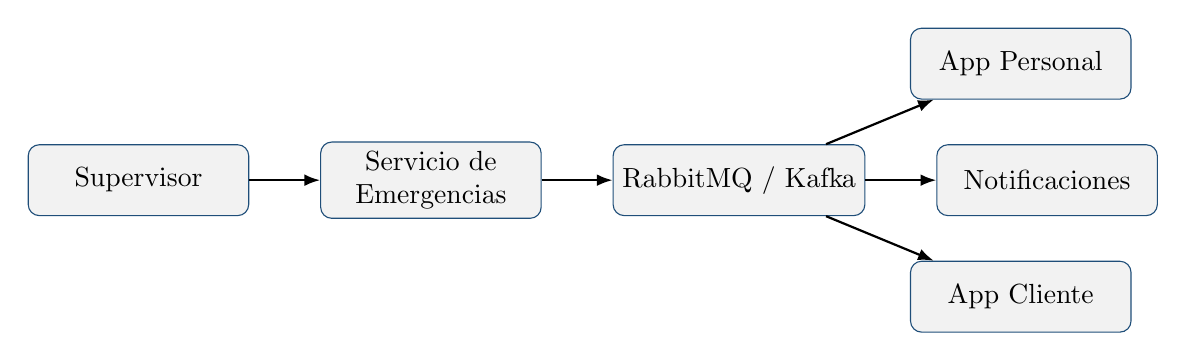
\begin{tikzpicture}[
box/.style={draw=azul,rounded corners,fill=gris,minimum width=2.8cm,minimum height=0.9cm,align=center},
arr/.style={-{Latex[length=2mm]},thick}
]
\node[box] (s) {Supervisor};
\node[box,right=9mm of s] (e) {Servicio de\\Emergencias};
\node[box,right=9mm of e] (q) {RabbitMQ / Kafka};
\node[box,above right=8mm of q] (p) {App Personal};
\node[box,below right=8mm of q] (c) {App Cliente};
\node[box,right=9mm of q] (n) {Notificaciones};
\draw[arr](s)--(e);
\draw[arr](e)--(q);
\draw[arr](q)--(p);
\draw[arr](q)--(c);
\draw[arr](q)--(n);
\end{tikzpicture}
\end{center}

\section{Relación entre interfaces y microservicios}

\begin{longtable}{p{4cm}p{4cm}p{6cm}}
\toprule
\textbf{Servicio} & \textbf{Interfaces} & \textbf{Responsabilidad}\\
\midrule
Entradas & Web Cliente, App Cliente & Compra, disponibilidad, validación y gestión.\\
Mercado Secundario & Web Cliente & Publicación, compra y transferencia.\\
Personal & Web Administrativo, App Personal & Empleados, turnos, asignaciones y asistencia.\\
Eventos & Web Administrativo, Web Cliente, Apps & Gestión y consulta de eventos.\\
Parqueaderos & Web Cliente, Web Administrativo, Apps & Reservas, espacios, cobros y ocupación.\\
Emergencias & Web Administrativo, App Personal, App Cliente & Activación, coordinación, alertas y seguimiento.\\
\bottomrule
\end{longtable}

\section{Resumen de decisiones arquitectónicas}

\begin{table}[H]
\centering
\small
\begin{tabular}{p{4cm}p{5cm}p{5cm}}
\toprule
\textbf{Decisión} & \textbf{Problema} & \textbf{Atributos}\\
\midrule
Microservicios & Separación de dominios y escalamiento & Escalabilidad, mantenibilidad, rendimiento\\
API Gateway & Punto central de acceso y seguridad & Seguridad, mantenibilidad\\
Balanceador & Distribución de solicitudes & Disponibilidad, rendimiento\\
Redis & Acceso rápido y bloqueo temporal & Consistencia, tiempo real, rendimiento\\
RabbitMQ/Kafka & Procesamiento asíncrono & Rendimiento, escalabilidad\\
BD por servicio & Evitar acoplamiento de datos & Mantenibilidad, escalabilidad\\
Notificaciones & Comunicación desacoplada & Rendimiento, tiempo real\\
Pasarela de pagos & Transacciones externas & Seguridad, consistencia\\
Interfaces especializadas & Adaptación al usuario & Usabilidad, portabilidad\\
\bottomrule
\end{tabular}
\caption{Resumen de decisiones arquitectónicas.}
\end{table}

\section{Conclusión}

La arquitectura propuesta conserva las decisiones fundamentales de la primera versión, pero las adapta a una definición más concreta del sistema: un portal web para clientes, un portal web administrativo y operativo, una aplicación móvil para clientes y una aplicación móvil para el personal.

La separación de interfaces permite que cada tipo de usuario tenga las funcionalidades que necesita, mientras que el backend mantiene la lógica de negocio centralizada en servicios independientes.

Los atributos de calidad prioritarios siguen siendo consistencia, disponibilidad, seguridad y rendimiento. Estos se soportan mediante microservicios, API Gateway, balanceador de carga, Redis, colas de mensajes, bases de datos independientes y servicios externos de pago y notificaciones.

La incorporación de aplicaciones móviles aumenta la importancia de tiempo real, usabilidad y portabilidad. Asimismo, la gestión de evacuación ante emergencias constituye un caso complejo adecuado para demostrar cómo las decisiones arquitectónicas responden a atributos de calidad concretos.

\end{document}
